\documentclass[11pt]{article}
\usepackage[margin=1in]{geometry}
\usepackage{amsmath}
\usepackage{booktabs}
\usepackage{graphicx}
\usepackage{hyperref}
\usepackage{longtable}
\usepackage{xurl}
\setlength{\emergencystretch}{3em}

\title{WEC2026 Goal-Scoring Prediction: Exploratory Data Analysis and\\Modeling Notes}
\author{Automated EDA report}
\date{April 26, 2026}

\begin{document}
\maketitle

\section{Executive Summary}
The WEC2026 data define a rare-event player-checkpoint prediction problem: estimate whether a player will score after a 15-minute checkpoint.
The modeling table contains 3,486 checkpoint observations, 203 positive examples, 31 fixtures, 307 players, and 869 player appearances.
The positive rate is only 5.82\%, so model evaluation should prioritize ranking and calibration metrics such as PR-AUC, ROC-AUC, Brier score, and lift in the top predicted risk bands rather than raw accuracy.

EDA indicates that the target is not uniformly distributed across football context.
Positive rates are highest for attackers and midfielders, higher before half time than after half time, and materially different across recent shot, speed, and pressure-related behavior.
The strongest descriptive correlations after temporal feature engineering are role and territory variables: attacker status, bottom-stage pass share, top-stage pass share, top-stage run share, pressure top share, and recent HSR ratio.
Grouped cross-validated model plots after removing proxy and future-known fields show that the best model by PR-AUC is XGBoost, while Random Forest has the best ROC-AUC and Brier score.
However, all associations remain modest because scoring is noisy, sparse, and heavily driven by match context.

\section{Dataset Inventory}
\begin{longtable}{lrrlp{0.34\linewidth}}
\toprule
Dataset & Rows & Columns & Player appearances & Role \\
\midrule
Checkpoints & 3,486 & 33 & 869 & Main modeling table \\
Passes & 29,795 & 7 & 959 & Technical event context \\
Runs & 35,133 & 10 & 968 & Physical event context \\
Shots & 780 & 12 & 453 & Attacking event context \\
Pressure & 12,185 & 10 & 923 & Pressed-action context \\
\bottomrule
\end{longtable}

The event files cover slightly more player appearances than the checkpoint table.
For modeling, event-derived features should be left joined to the 869 checkpoint-table player appearances and filtered by checkpoint time to avoid using future events.
Among checkpoint-table appearances, pass events cover 99.9\%, run events cover 99.0\%, pressure events cover 97.1\%, and shot events cover 50.4\%.

\section{Data Quality}
The main checkpoint table has no missing values in the supplied CSV.
The pass table is nearly complete, with 0.14\% missing addressees and 0.19\% missing stage values.
The shot table has 72.4\% missing block-player IDs and 99.9\% missing own-goal-player IDs; these fields should be interpreted as event indicators rather than numeric identifiers requiring imputation.
The pressure table has meaningful missingness: 5.3\% missing addressees and 47.5\% missing pass angles.
Missing pass angle should receive its own indicator because it likely separates non-pass or non-measured pressured actions from ordinary passes.

\begin{longtable}{lrr}
\toprule
Field & Missing count & Missing share \\
\midrule
\texttt{pass.addressee\_player\_appearance\_id} & 41 & 0.14\% \\
\texttt{pass.stage} & 57 & 0.19\% \\
\texttt{shot.block\_player\_appearance\_id} & 565 & 72.44\% \\
\texttt{shot.own\_goal\_player\_appearance\_id} & 779 & 99.87\% \\
\texttt{pressure.addressee\_player\_appearance\_id} & 649 & 5.33\% \\
\texttt{pressure.pass\_angle} & 5,793 & 47.54\% \\
\texttt{pressure.stage} & 14 & 0.11\% \\
\bottomrule
\end{longtable}

\section{Target Distribution}
The target \texttt{scored\_after} is encoded as 0/1.
There are 203 positive checkpoints and 3,283 negative checkpoints, for a base rate of 5.82\%.
Twenty-seven of 31 fixtures contain at least one positive checkpoint; among positive fixtures, the number of positive checkpoint rows ranges from 1 to 16 with a median of 6.
This confirms that fixture-grouped validation is necessary: random row splits would leak match state and repeated player appearances across train and validation folds.

\begin{longtable}{lrrr}
\toprule
Segment & Observations & Positives & Positive rate \\
\midrule
All checkpoints & 3,486 & 203 & 5.82\% \\
Home players & 1,744 & 91 & 5.22\% \\
Away players & 1,742 & 112 & 6.43\% \\
\bottomrule
\end{longtable}

\subsection{Target by Match Time}
Positive rates decline through the match checkpoints.
The first checkpoint, H1 15, has the highest positive rate at 8.96\%, while the regular second-half checkpoints are below 4.0\%.
This does not necessarily mean that early minutes cause goals; it can also reflect how \texttt{scored\_after} is defined, because early checkpoints have a longer remaining horizon.
Checkpoint time must therefore be included as a core feature, and any comparison of player behavior should control for checkpoint.

\begin{longtable}{lrrr}
\toprule
Checkpoint & Observations & Positives & Positive rate \\
\midrule
H1 15 & 681 & 61 & 8.96\% \\
H1 30 & 680 & 48 & 7.06\% \\
H1 45 & 680 & 39 & 5.74\% \\
H2 15 & 680 & 27 & 3.97\% \\
H2 30 & 680 & 25 & 3.68\% \\
H2 45 & 43 & 2 & 4.65\% \\
ET1 15 & 42 & 1 & 2.38\% \\
\bottomrule
\end{longtable}

\subsection{Target by Position}
Position is one of the clearest contextual splits.
Attackers have a 12.52\% positive rate, midfielders 6.73\%, defenders 3.05\%, and goalkeepers have no positive examples.
Goalkeepers should either be excluded from scorer-specific models or handled by a deterministic near-zero prior; keeping them in an unconstrained classifier may mostly teach the model an obvious position rule.

\begin{longtable}{lrrr}
\toprule
Position & Observations & Positives & Positive rate \\
\midrule
Attacker & 615 & 77 & 12.52\% \\
Midfielder & 1,307 & 88 & 6.73\% \\
Defender & 1,246 & 38 & 3.05\% \\
Goalkeeper & 318 & 0 & 0.00\% \\
\bottomrule
\end{longtable}

\begin{figure}[htbp]
\centering
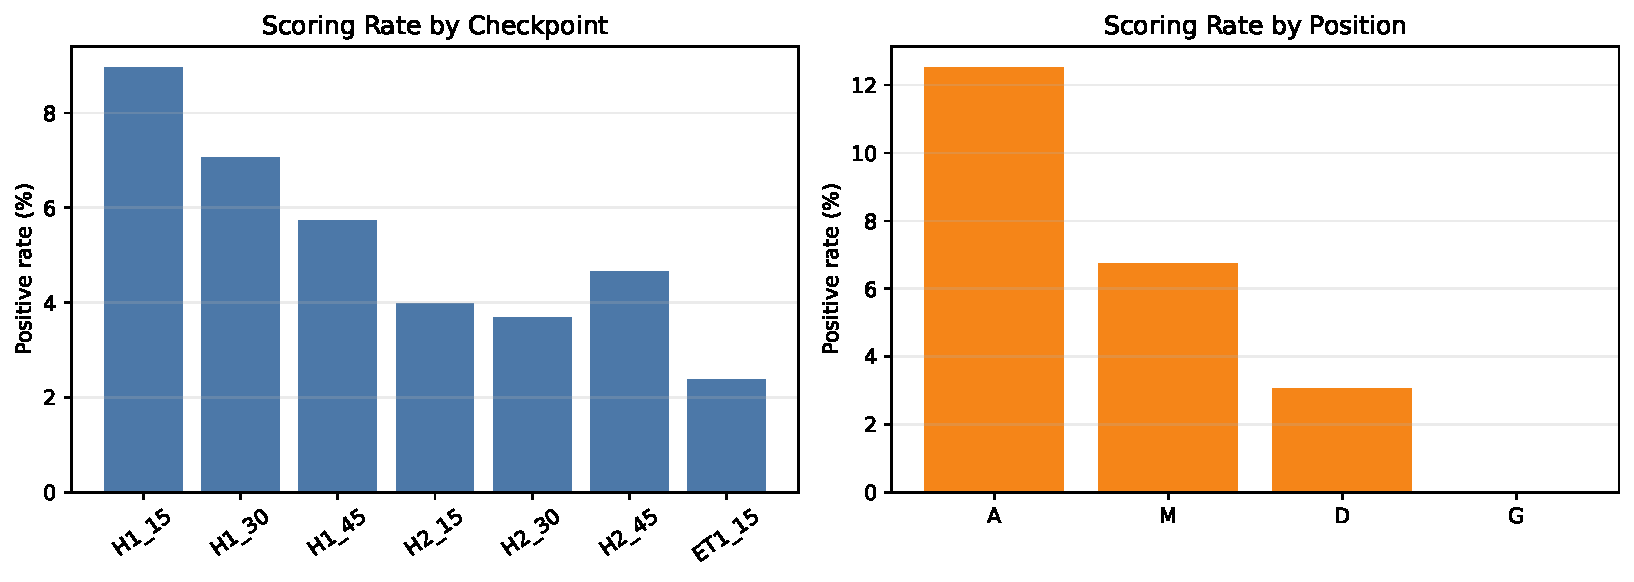
\includegraphics[width=\linewidth]{figures/target_rates.pdf}
\caption{Target rate by checkpoint and player position. The visual pattern confirms that time horizon and tactical role are first-order controls for any scorer model.}
\end{figure}

\section{Checkpoint Feature EDA}
The checkpoint table contains both recent 15-minute features and cumulative features.
Recent shot and speed measures are sparse but informative.
For positive rows, \texttt{last15\_shots} averages 0.271 compared with 0.161 for negative rows, and \texttt{last15\_peak\_speed} averages 7.88 compared with 7.24.
Cumulative shooting also separates positives from negatives: \texttt{cumul\_shots\_on\_target} averages 0.241 for positives and 0.150 for negatives.

\begin{longtable}{lrrr}
\toprule
Feature & Positive mean & Negative mean & Difference \\
\midrule
\texttt{last15\_peak\_speed} & 7.882 & 7.241 & 0.641 \\
\texttt{last15\_mean\_max\_speed} & 6.654 & 6.191 & 0.464 \\
\texttt{last15\_shots\_top\_third} & 0.266 & 0.156 & 0.110 \\
\texttt{last15\_shots} & 0.271 & 0.161 & 0.109 \\
\texttt{last15\_hsr} & 7.271 & 6.397 & 0.874 \\
\texttt{cumul\_shots} & 0.591 & 0.418 & 0.173 \\
\texttt{cumul\_shots\_on\_target} & 0.241 & 0.150 & 0.091 \\
\texttt{cumul\_hsr} & 16.507 & 18.246 & -1.738 \\
\bottomrule
\end{longtable}

The marginal effects should be interpreted cautiously.
The largest point-biserial correlations with the target are only about 0.08--0.13, which is expected for a rare football scoring event.
These features are useful as weak signals, not as standalone rules.
The negative contrast for cumulative HSR suggests that accumulated running volume is not equivalent to attacking threat; position, minutes played, tactical role, and fatigue must be modeled jointly.

\subsection{Feature Correlations}
Figure 2 shows the largest absolute correlations with the target after fold-safe temporal feature engineering.
The strongest positive correlations are attacker status and top-stage territorial indicators.
The strongest negative correlations are bottom-stage possession and time-exposure variables.
The leading values are listed below.

\begin{figure}[htbp]
\centering
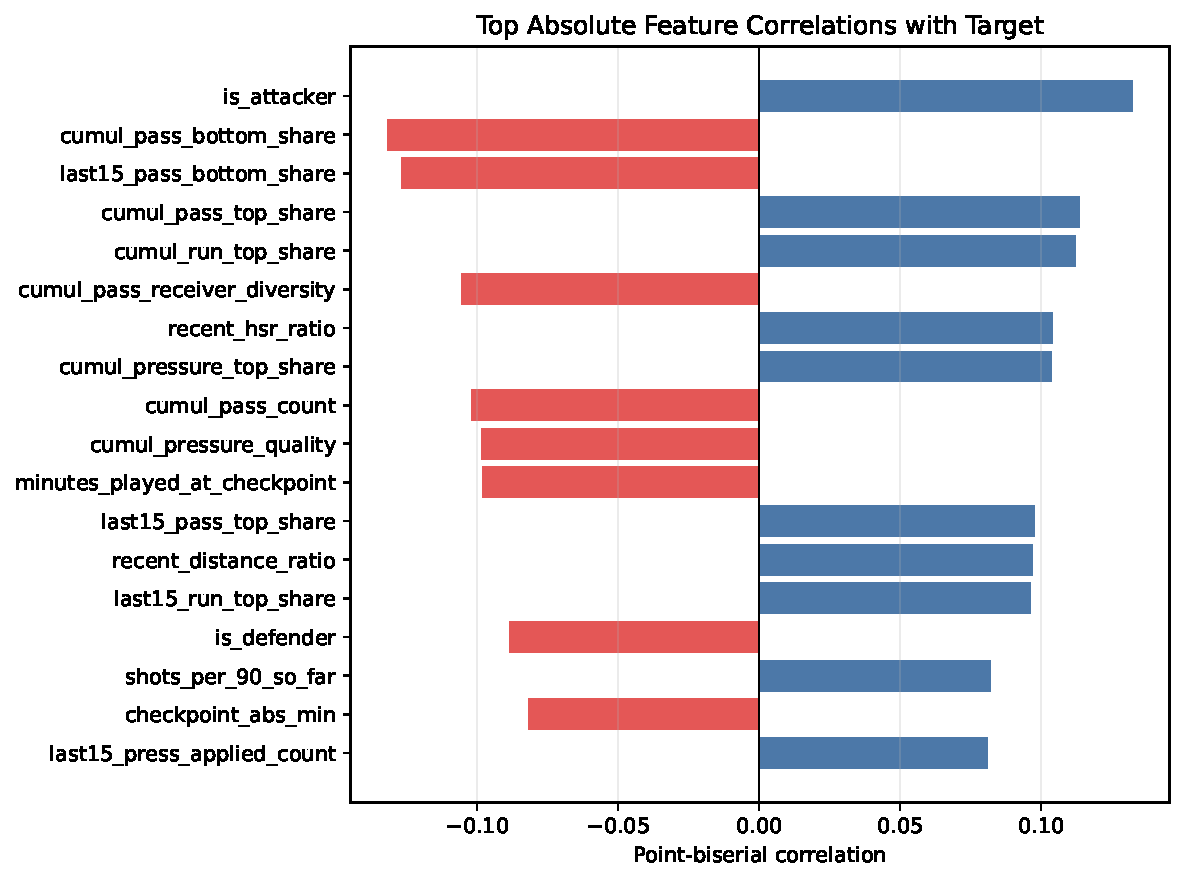
\includegraphics[width=\linewidth]{figures/feature_correlations.pdf}
\caption{Top absolute feature correlations with \texttt{scored\_after}. These are descriptive associations, not causal effects.}
\end{figure}

\begin{longtable}{lr}
\toprule
Feature & Correlation with target \\
\midrule
\texttt{is\_attacker} & 0.132 \\
\texttt{cumul\_pass\_bottom\_share} & -0.132 \\
\texttt{last15\_pass\_bottom\_share} & -0.127 \\
\texttt{cumul\_pass\_top\_share} & 0.114 \\
\texttt{cumul\_run\_top\_share} & 0.112 \\
\texttt{cumul\_pass\_receiver\_diversity} & -0.106 \\
\texttt{recent\_hsr\_ratio} & 0.104 \\
\texttt{cumul\_pressure\_top\_share} & 0.104 \\
\bottomrule
\end{longtable}

\subsection{Sparsity and Outliers}
Shot features are highly zero-inflated.
In the last-15-minute window, 85.2\% of rows have zero shots and 94.3\% have zero shots on target.
Cumulative shots are also zero for 70.9\% of rows.
Tree models can handle this sparsity, but linear models should use explicit zero indicators or count transformations.

Distance features are right-skewed.
\texttt{last15\_distance} has a median of 107.20, a mean of 367.13, and a maximum of 8,028.31.
\texttt{cumul\_distance} has a median of 277.84, a mean of 969.21, and a maximum of 25,667.77.
These maxima are much larger than the interquartile range, so robust scaling, clipping, or logarithmic transformations should be tested.

\section{Event-Level EDA}
\subsection{Passing}
The pass table contains 29,795 events with an overall accuracy rate of 83.78\%.
Nearly half of all passes occur in the middle stage.
Accuracy falls as the ball moves toward the top stage: 88.16\% in the middle, 82.48\% in the bottom, and 76.27\% in the top.
This stage gradient supports constructing zone-specific passing features rather than using only total pass counts.

\begin{longtable}{lrr}
\toprule
Pass stage & Events & Accuracy \\
\midrule
Middle & 14,369 & 88.16\% \\
Bottom & 8,733 & 82.48\% \\
Top & 6,636 & 76.27\% \\
Missing & 57 & 50.88\% \\
\bottomrule
\end{longtable}

\subsection{Running}
The run table contains 35,133 events: 80.88\% high-speed runs and 19.12\% sprints.
The median run distance is 12.07, while the mean is 47.93 and the maximum is 1,694.01.
The distance distribution is therefore highly skewed at the event level as well as at the checkpoint aggregate level.
Useful derived features include sprint share, HSR-to-sprint ratio, maximum speed above positional baseline, and recent-versus-cumulative acceleration in running volume.

\subsection{Shots}
The shot table contains 780 shots.
Most shots are right-footed or left-footed, 95.90\% occur in the top stage, 77.82\% are under pressure, and 27.56\% are blocked.
Because the shot file is limited and does not expose final shot outcome as a modeling label, its best use is contextual: recent shot count, shot pressure share, blocked-shot involvement, and top-stage shooting volume.

\begin{longtable}{lrr}
\toprule
Shot attribute & Count & Share \\
\midrule
Right foot & 404 & 51.79\% \\
Left foot & 271 & 34.74\% \\
Header & 104 & 13.33\% \\
Regular play & 543 & 69.62\% \\
Corner kick & 84 & 10.77\% \\
Counter attack & 60 & 7.69\% \\
Under pressure & 607 & 77.82\% \\
Blocked & 215 & 27.56\% \\
\bottomrule
\end{longtable}

\subsection{Pressure}
The pressure table contains 12,185 events.
The pass/action accuracy rate under pressure is 57.04\%, far below the ordinary pass accuracy rate.
Turnovers account for 39.09\% of pressured actions, backward passes 26.37\%, forward passes 18.66\%, carries 8.45\%, and lateral passes 7.43\%.
Pressure effects vary by stage: top-stage pressured actions have a 42.81\% turnover rate and 51.10\% accuracy, while middle-stage pressured actions have a 35.16\% turnover rate and 62.42\% accuracy.

\begin{longtable}{lrrr}
\toprule
Pressure stage & Events & Turnover rate & Accuracy \\
\midrule
Middle & 5,492 & 35.16\% & 62.42\% \\
Top & 4,076 & 42.81\% & 51.10\% \\
Bottom & 2,603 & 41.53\% & 55.24\% \\
Missing & 14 & 42.86\% & 7.14\% \\
\bottomrule
\end{longtable}

\begin{figure}[htbp]
\centering
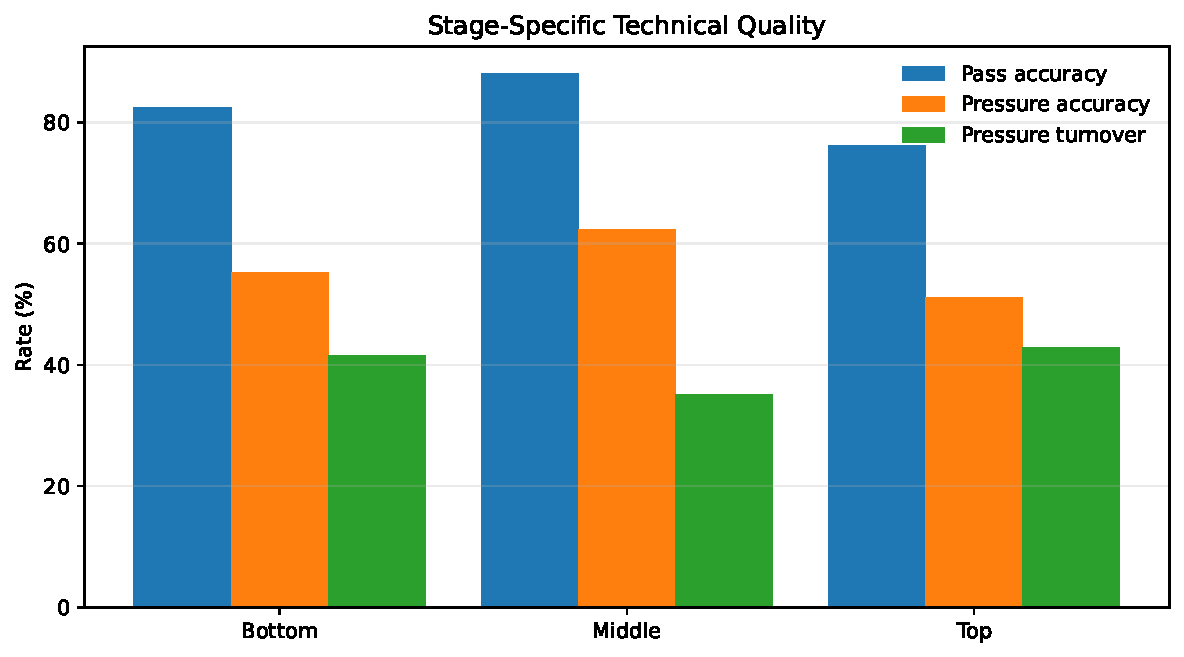
\includegraphics[width=0.78\linewidth]{figures/event_stage_quality.pdf}
\caption{Stage-specific event quality. Top-stage actions are more threatening but less secure: ordinary pass accuracy drops and pressure turnover rates rise.}
\end{figure}

\section{Methodology}
The analysis treats each player-checkpoint row as an information set: at checkpoint time, the model may use static pre-match context, player role, home/away status, elapsed time, and event aggregates observed up to that checkpoint.
The target is \texttt{scored\_after}, so the task is a rare-event ranking and probability-estimation problem rather than a balanced classification problem.

Event features are built with a fold-safe temporal transformer.
Within each cross-validation fold, reference quantities such as zone threat values, pressure turnover baselines, and positional baselines are fitted only on the training fixtures and then applied to validation fixtures.
For each checkpoint, pass, run, shot, and pressure events are joined by player appearance id and filtered using both period and minute.
This is necessary because event minutes are period-relative and overlap across halves: first-half stoppage time can exceed minute 45, while second-half events restart from low minute values.
Using minute alone would therefore either drop valid past events or admit future events from another period.

Feature families include recent and cumulative physical workload, shot involvement, stage-weighted passing, expected-threat-style pass progression, pressure resistance, pressing applied, role indicators, and time controls.
Recent windows use the previous 15 minutes within the absolute period-aware match clock, while cumulative features use events from the player's appearance start up to the checkpoint.
Categorical variables are one-hot encoded inside each fold after temporal feature construction.

Model comparison uses stratified grouped cross-validation with \texttt{fixture\_id} as the group.
This prevents rows from the same match from appearing in both training and validation, which would otherwise leak shared match state, opponent context, and repeated player appearances.
The reported models are XGBoost, Random Forest, Extra Trees, and balanced logistic regression.
Evaluation emphasizes PR-AUC, ROC-AUC, and Brier score because positives are sparse and calibrated probabilities are more useful than default-threshold labels.

\section{Data Leakage and Proxy Features}
The main leakage risk in this project is temporal: event-derived features must not use passes, runs, shots, or pressured actions that occur after a checkpoint.
All report figures and model summaries use the temporal feature builder with fixture-grouped folds, and event aggregates are filtered to each player appearance before the checkpoint period and minute.
Validation is grouped by \texttt{fixture\_id} to avoid evaluating on rows from the same match that appear in training.

\texttt{minute\_out} and \texttt{subbed} are excluded from the modeling feature sets.
Although they are present in the final checkpoint file, they are not necessarily known at an earlier checkpoint: whether and when a player is eventually substituted can reveal future tactical or physical information.
They remain useful for quality checks, for example filtering invalid off-pitch rows, but they should not be supplied to the classifier.

\texttt{jersey\_number} was also removed from the modeling feature sets.
It is known before the match and is therefore not classical target leakage, but it is a weak proxy feature: it can encode squad role, attacking position, club numbering conventions, or player identity patterns that may not generalize to the hidden test set.
It also has no meaningful ordinal interpretation, so treating it as a numeric variable can create arbitrary splits.
The model already has cleaner role and tactical signals through position, formation, top-stage activity, shots, pressure metrics, and running intensity.

The exclusions are implemented centrally in \texttt{src/temporal\_features.py} through the non-model column list used by \texttt{modeling\_columns()} and by the feature-set factory.
The validation helper also supports period-aware temporal merges, so future-event checks use period and minute together.

\section{Grouped-CV Model Plots and Feature Importance}
The plotting script trains four candidate models with fixture-grouped stratified cross-validation using the temporal feature builder: XGBoost, Random Forest, Extra Trees, and balanced logistic regression.
The script is reproducible with:
\[
\texttt{.venv/bin/python scripts/create\_eda\_plots.py}
\]
It writes figures and supporting CSV files to \texttt{reports/figures/}.

\begin{longtable}{lrrr}
\toprule
Model & ROC-AUC & PR-AUC & Brier \\
\midrule
XGBoost & 0.652 & 0.124 & 0.085 \\
Extra Trees & 0.669 & 0.113 & 0.061 \\
Random Forest & 0.683 & 0.110 & 0.058 \\
Logistic regression & 0.584 & 0.089 & 0.188 \\
\bottomrule
\end{longtable}

\begin{figure}[htbp]
\centering
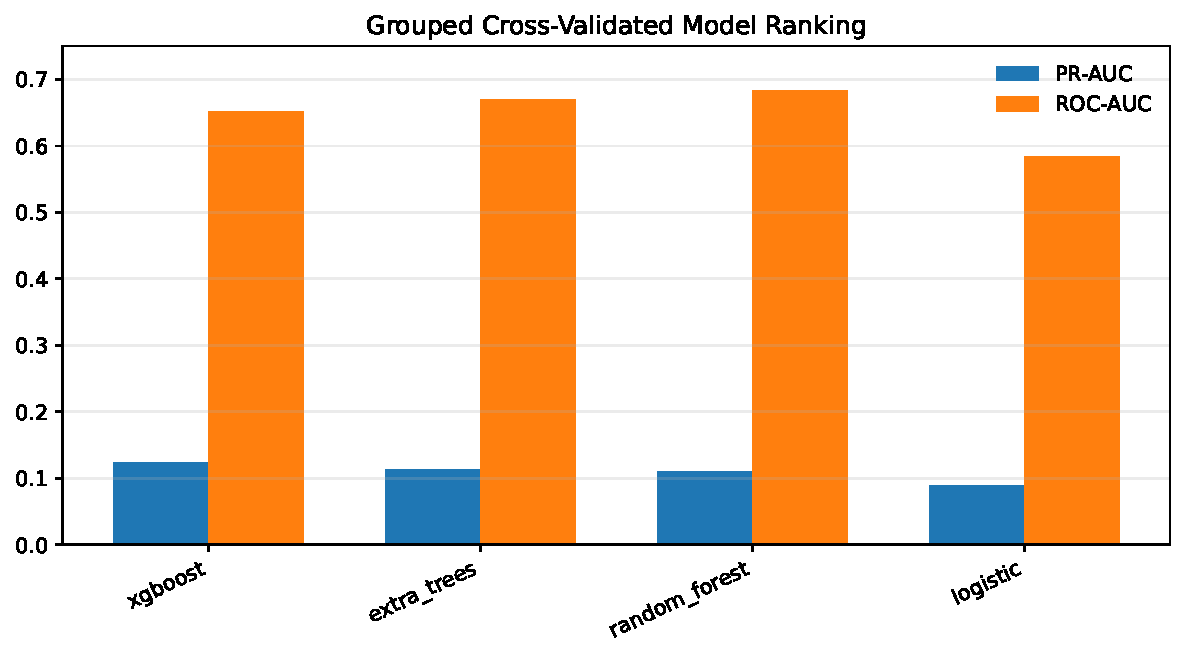
\includegraphics[width=0.82\linewidth]{figures/model_comparison.pdf}
\caption{Grouped cross-validated model ranking after excluding proxy and future-known fields. XGBoost gives the best PR-AUC, while Random Forest gives the best ROC-AUC and Brier score among the tested models.}
\end{figure}

The best two models by PR-AUC are XGBoost and Extra Trees.
Their feature importance profiles agree on several themes: territorial possession, bottom-vs-top stage shares, pressure quality, player role, and recent physical intensity.
This agreement is more useful than any single importance rank, because impurity-based importances can be biased toward continuous or high-cardinality features.

\begin{figure}[htbp]
\centering
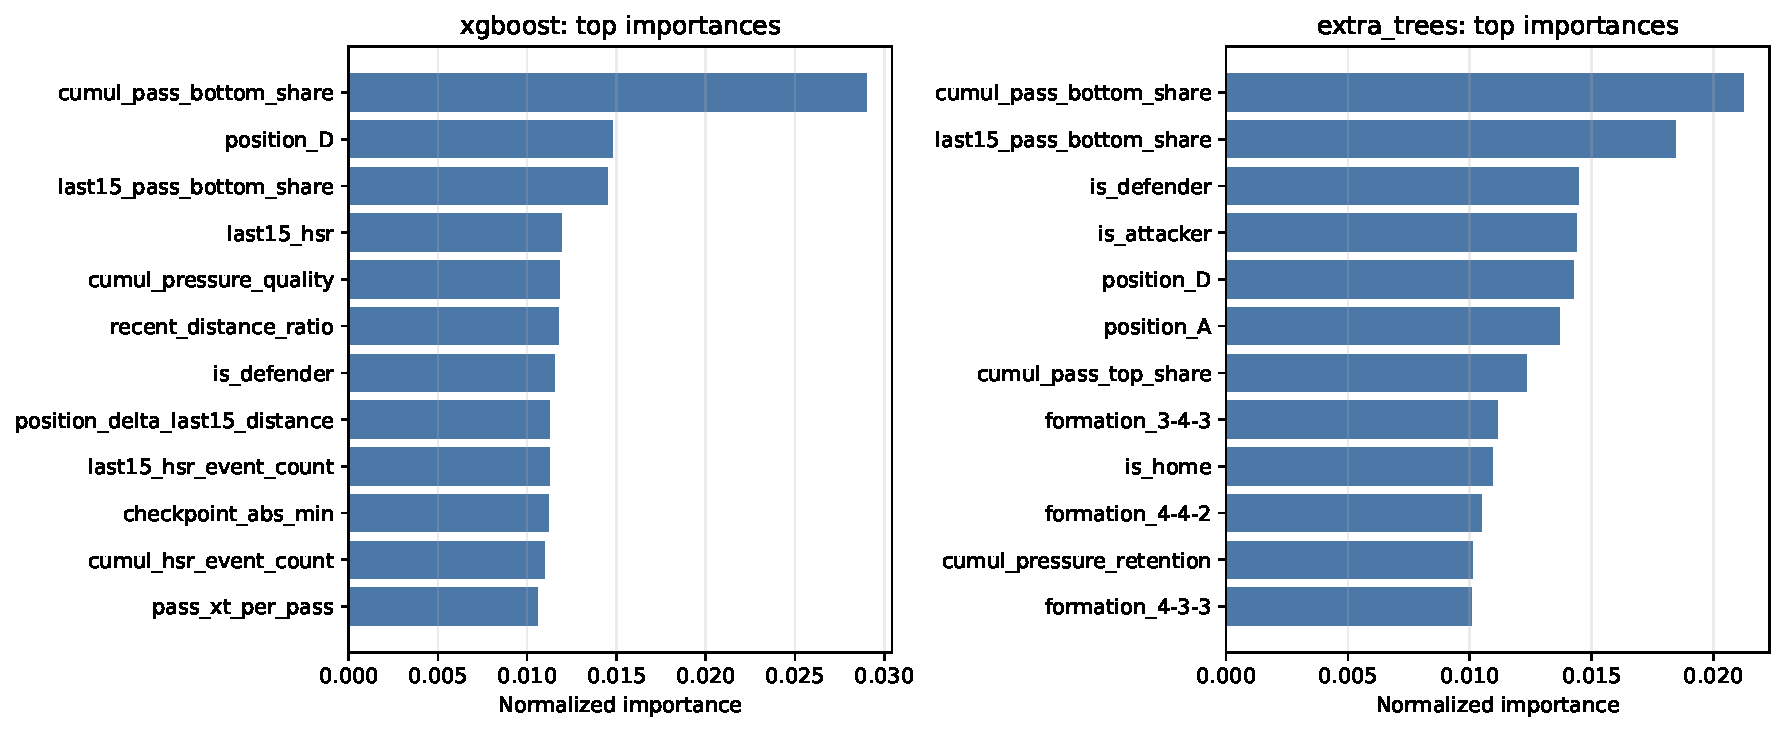
\includegraphics[width=\linewidth]{figures/model_feature_importance.pdf}
\caption{Top normalized feature importances for the two best PR-AUC models in the plotting run.}
\end{figure}

\begin{longtable}{llr}
\toprule
Model & Feature & Normalized importance \\
\midrule
XGBoost & \texttt{cumul\_pass\_bottom\_share} & 0.031 \\
XGBoost & \texttt{position\_D} & 0.015 \\
XGBoost & \texttt{last15\_pass\_bottom\_share} & 0.015 \\
XGBoost & \texttt{last15\_hsr} & 0.012 \\
XGBoost & \texttt{cumul\_pressure\_quality} & 0.012 \\
XGBoost & \texttt{recent\_distance\_ratio} & 0.012 \\
Extra Trees & \texttt{cumul\_pass\_bottom\_share} & 0.021 \\
Extra Trees & \texttt{last15\_pass\_bottom\_share} & 0.018 \\
Extra Trees & \texttt{is\_defender} & 0.014 \\
Extra Trees & \texttt{is\_attacker} & 0.014 \\
Extra Trees & \texttt{position\_D} & 0.014 \\
Extra Trees & \texttt{position\_A} & 0.014 \\
\bottomrule
\end{longtable}

The feature-importance plots sharpen the EDA conclusions.
First, bottom-stage pass share is consistently negative in correlation and highly important in both nonlinear models, suggesting that possession far from goal is a strong proxy for lower immediate scoring risk.
Second, top-stage pass and run shares are positively correlated with scoring, supporting the use of territory-weighted event aggregates.
Third, pressure variables matter: \texttt{cumul\_pressure\_quality}, top pressure share, and pressure angle summaries appear in either correlation or importance views.
Finally, after removing \texttt{jersey\_number}, role information is still captured by explicit and interpretable variables such as \texttt{position\_A}, \texttt{position\_D}, \texttt{is\_attacker}, and \texttt{is\_defender}.

\section{Modeling Implications}
The validation design should be fixture grouped, and ideally stratified by target where possible.
Rows from the same fixture share game state, opponent strength, tempo, and repeated player appearances; random splits would overstate performance.
Because there are only 203 positives, fold-level variance will be high, and a single holdout split is not enough for stable conclusions.

Feature engineering should be explicitly temporal.
For every checkpoint, event features should use only events from the player's appearance up to that checkpoint.
Useful feature families include recent and cumulative shot counts, top-stage shot share, recent speed and HSR intensity, pass accuracy by stage, pressure turnover rate, pressure escape rate, and recent-versus-cumulative workload ratios.
Checkpoint time, position, formation, home/away status, and known minutes played so far should be retained as control variables.
Future-known substitution fields such as \texttt{minute\_out} and \texttt{subbed} should remain excluded from model inputs.

The class imbalance requires threshold-aware evaluation.
A default 0.5 threshold is unlikely to be appropriate.
Recommended reporting includes PR-AUC, ROC-AUC, Brier score, calibration plots, recall at fixed precision, and lift among the top 5\% or top 10\% predicted-risk checkpoints.
For competition usage, predicted probabilities are more valuable than hard labels.

\section{Conclusions}
The data contain meaningful football signal, but it is weak, sparse, and context dependent.
The most reliable EDA patterns are positional scoring propensity, the declining target rate across later checkpoints, territorial possession, recent attacking involvement, recent speed intensity, and pressure-stage effects.
Passing and pressure events add tactical context that is not present in the checkpoint table, especially because pass accuracy and pressure turnover rates change strongly by stage.

The main modeling risk is leakage from future events or from fixture-level random splits.
The second major risk is overfitting: 203 positives are not enough to support very high-dimensional feature sets without regularization, grouped validation, and careful calibration.
The plot-based model comparison suggests that a tuned XGBoost model is the best immediate ranking baseline, while Random Forest is a useful calibration and robustness comparator.
The strongest next modeling baseline is therefore a grouped cross-validated gradient-boosted tree model with temporally filtered event aggregates, class weighting, calibrated probabilities, and a simple sparse linear model as a sanity-check comparator.

\begin{thebibliography}{9}
\bibitem{singh2019xt}
Singh, K. (2019). Introducing Expected Threat (xT). StatsBomb.
\url{https://statsbomb.com/articles/soccer/introducing-expected-threat-xt/}

\bibitem{chen2016xgboost}
Chen, T. and Guestrin, C. (2016). XGBoost: A scalable tree boosting system.
In \emph{Proceedings of the 22nd ACM SIGKDD International Conference on Knowledge Discovery and Data Mining}, 785--794.

\bibitem{breiman2001random}
Breiman, L. (2001). Random forests. \emph{Machine Learning}, 45, 5--32.

\bibitem{niculescu2005probabilities}
Niculescu-Mizil, A. and Caruana, R. (2005). Predicting good probabilities with supervised learning.
In \emph{Proceedings of the 22nd International Conference on Machine Learning}, 625--632.

\bibitem{fawcett2006roc}
Fawcett, T. (2006). An introduction to ROC analysis. \emph{Pattern Recognition Letters}, 27(8), 861--874.
\end{thebibliography}

\end{document}
